\section*{Introduction}

What a nice template\footnote{I did it myself!} for \citep{Rougier:2017}.

\subsection*{Figures}
\begin{figure}[htbp]
   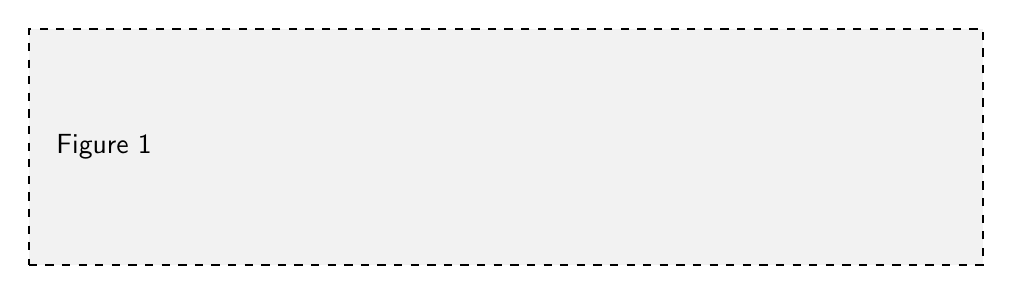
\begin{tikzpicture}
     \node[draw, fill=black!5, dashed, thick,
       text width=.98\textwidth, minimum height=3cm] at (0,0) {~~\sf Figure 1};
   \end{tikzpicture}
    \captionof{figure}{Figure caption}
    \label{fig:1}
\end{figure}

\begin{table}[htbp]
\begin{minipage}{.45\textwidth}
  \begin{tabularx}{\textwidth}{|XX|}
      \hline
      \bfseries Header 1 & \bfseries Header 2\\
      \hline
      Item 1 & Item 2\\
      Item 1 & Item 2\\
      Item 1 & Item 2\\
      \hline
    \end{tabularx}
    \captionof{table}{Table caption}
    \label{tab:1}
\end{minipage}
\hfill
\begin{minipage}{.45\textwidth}
  \begin{tabularx}{\textwidth}{|XX|}
      \hline
      \bfseries Header 1 & \bfseries Header 2\\
      \hline
      Item 1 & Item 2\\
      Item 1 & Item 2\\
      Item 1 & Item 2\\
      \hline
    \end{tabularx}
    \captionof{table}{Table caption}
    \label{tab:2}
\end{minipage}
\end{table}


The well known Pythagorean theorem \(x^2 + y^2 = z^2\) was proved to be invalid
for other exponents.  Meaning equation \eqref{eq:1} has no integer solutions:
%%
\begin{equation}
  \label{eq:1}
  x^n + y^n = z^n
\end{equation}


\begin{lstlisting}[language=python, caption={Listing caption}, label={lst:1}]
# Standard import
import this

text = "Some text"
\end{lstlisting}


\section*{Conclusion}

This is a short article.
